% Emacs settings: -*-mode: latex; TeX-master: "manual.tex"; -*-

\chapter{Source components}
\label{c:source}
\index{Sources|textbf}
\index{Library!Components!sources}

\MCX\ contains a number of different source components,
and any simulation will usually contain exactly one of these sources.
The main function of a source is to determine a set of initial
parameters $({\bf r}, {\bf v}, t)$
for each neutron ray. This is done by Monte Carlo choices from
suitable distributions. For example, in most present sources
the initial position is
found from a uniform distribution over the source surface,
which can be chosen to be either circular or rectangular.
The initial neutron velocity is selected within an interval
of either the corresponding energy or the corresponding wavelength.
Polarization is not relevant for sources,
and we initialize the neutron average spin to zero: ${\bf s}=(0,0,0)$.

For time-of-flight sources, the choice of the emission time, $t$,
is being made on basis of detailed analytical expressions.
For other sources, $t$ is set to zero.
In the case one would like to use a steady state source
with time-of-flight settings,
the emission time of each neutron ray should be determined using
a Monte Carlo choice. This may be achieved by
the \verb+EXTEND+ keyword in the instrument description source
as in the example below:\index{Keyword!EXTEND}

\begin{verbatim}
  TRACE

  COMPONENT MySource=Source_gen(...) AT (...)
  EXTEND
  %{
    t = 1e-3*randpm1(); /* set time to +/- 1 ms */
  %}
\end{verbatim}

\subsection{Photon flux and Brilliance}
\label{s:xray-flux}
The flux of the sources deserves special attention. The total
intensity is defined as the sum of weights of all emitted xrays
during one simulation
(the unit of total photon weight is thus xrays per second).
The flux, $\psi$, at an instrument is defined as intensity per area perpendicular
to the beam direction.

The source flux, $\Phi$, is defined in different units:
the number of photon rays emitted per second from a
1~cm$^2$ area on the source surface,
with direction within a 1~ster.\ solid angle,
and with wavelength within a 1 {\AA} interval.
The total intensity of real neutrons emitted towards a given diaphragm
(units: n/sec) is therefore (for constant $\Phi$):
\begin{equation}
I_{\rm total} = \Phi A \Delta\Omega \Delta\lambda ,
\end{equation}
where $A$ is the source area, $\Delta\Omega$ is the solid angle of the
diaphragm as seen from the source surface, and $\Delta\lambda$ is the
width of the wavelength interval in which neutrons are emitted (assuming
a uniform wavelength spectrum).

The simulations are performed so that detector intensities
are independent of the number of neutron histories simulated
(although more neutron histories will give better statistics).
If $N_{\rm sim}$ denotes the number of
xray histories to simulate, the initial photon weight $p_0$ must be set to
\begin{equation}
\label{proprule}
p_0 = \frac{N_{\rm total}}{N_{\rm sim}} =
    \frac{\Phi(\lambda)}{N_{\rm sim}} A \Omega \Delta\lambda ,
\end{equation}
where the source flux is now given a $\lambda$-dependence.

As a start, we recommend new \MCX\ users to use the
{\bf Source\_simple} component.
Slightly more realistic sources are {\bf Source\_Maxwell\_3} for
continuous sources or {\bf Moderator} for time-of-flight sources.

Optimizers can dramatically improve the statistics, but may occasionally
give wrong results, due to misleaded optimization.
You should always check such simulations with (shorter) non-optimized ones.

Other ways to speed-up simulations are to read events from a file.
See section \ref{sources-seealso} for details.

\begin{figure}
  \begin{center}
    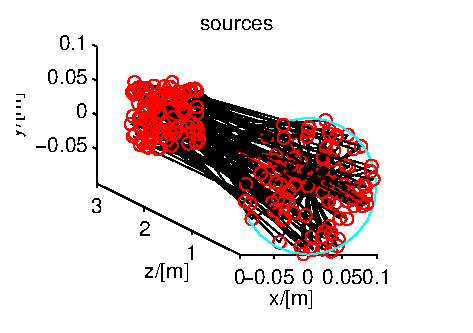
\includegraphics[width=0.75\textwidth]{figures/sources.eps}
  \end{center}
\caption{A circular source component (at z=0) emitting photon rays randomly, either from a model, or from a data file.}
\label{f:source}
\end{figure}

\newpage
\section{Source\_pt: A mathematical point emitting photons with a spectrum either uniform, gaussian or generated from a datafile}
\label{source-pt}
\index{Sources!Point source}
\component{Source\_pt}{System}{$dist$,$focus\_xw$,$focus\_yh$}{$\lambda_0$,${\rm d}\lambda$,$E$, $dE$, $spectrum\_file$, $incoherent$,$phase$}

The simplest source model, where a mathematical point source at $(0,0,0)$ emits photons. The wavevector of the emitted photons
is picked randomly in a defining aperture $focus\_xw$ by $focus\_yh$ m at $(0,0,dist)$. 
Please note that this aperture is merely a
virtual aperture used to reduce the sampling space. This has a few
implications: Other components may be placed without reference to the aperture,
but if the aperture does not fill the full acceptance window of subsequent
components your simulations will be biased. The aperture is simply there to provide efficient sampling.

If a $spectrum\_file$ is not supplied, the xray
is given a weight which is the total wavelength-integrated intensity downscaled
by the
solid subtended by the definning aperture.

If a $spectrum\_file$ \emph{is} supplied, a slightly different strategy is adopted. In this case the
wavelength/energy range implied by the datafile is sampled unformly and each ray is assigned
a weight corresponding to the intensity indicated by linear interpolation between datapoints
at that wavelength. This implies an oversampling of weak parts of the intensity spectrum.

Currently only completely coherent or fully incoherent beams are supported. If
$phase$ is specified emitted photons be assigne dthat phase, otherwise it is
chosen randomly.


\section{Source\_flat: A flat surface emitting photons with a spectrum either uniform, gaussian or generated from a datafile}
\label{source-flat}
\index{Sources!Flat surface source}
\component{Source\_flat}{System}{$d$,$w$,$h$}{$r$,$x_{width}$,$y_{height}$,$d$, $\lambda_0$,${\rm d}\lambda$, $spectrum\_file$, $incoherent$,$phase$}

A simple source model, with a flat surface emitting photons. The surface in the
$xy$-plane is specified as a rectangle with dimensions
$x_{width}\times y_{height}$ m, or as a circle w radius,$r$. 
The initial xray position is chosen randomly in the source surface --- its
wavevector is chosen randomly (exactly as in the case of \verb+Source\_pt+ (section \ref{source_pt}) in the defining aperture with height $h$ and
width $w$ placed at $(0,0,dist)$. 

Just as for \verb+Source\_pt+ the aperture is for efficiency purposes and, if misused, may cause biasing

A spectrum file may be supplied as for \verb+Source\_pt+.

Currently only fully coherent or incoherent beams are supported. If $phase$ is set (and not $randomphase$ which takes precedence) a phase is set such that a photon emitted from $(x,y,0)$ will be in phass with a photon at $(0,0,0)$, which has the phase $phase$..


\section{Source\_div: A continuous source with specified divergence}
\label{source-div}
\index{Sources!Continuous source with specified divergence}

\component{Source\_div}{System}{ $w$, $h$, $\delta_h$, $\delta_v$, $E_0$, $\Delta E$}{$\lambda_0$, $\Delta\lambda$, gauss}{Validated. t=0}

{\bf Source\_div} is a rectangular source, $w \times h$, which emits a
beam of a specified divergence around the direction of the $z$ axis.
The beam intensity is uniform over
the whole of the source, and the energy (or wavelength) distribution
of the beam is uniform over the specified energy range
$E_0 \pm \Delta E$ (in meV), or alternatively
the wavelength range $\lambda_0 \pm \delta\lambda$ (in \AA ).

The source divergences are $\delta_h$ and $\delta_v$ (FWHM in degrees).
If the \verb+gauss+ flag is set to 0 (default),
the divergence distribution is uniform, otherwise it is Gaussian.

This component may be used as a simple model of the
beam profile at the end of a guide or at the sample position.



\section{Source\_gaussian: the model has a gaussian distribution of intensity}
\label{source-gaussian}
\index{Sources!Source\_gaussian}
\component{Source\_gaussian}{System}{$d$,$w$,$h$}{$sig_x$,$sig_y$,$sigPr_x$,$sigPr_y$,$flux$,$dist$, $\lambda_0$,$\lambda 0$,$E0$,$dE$,$phase$}

A simplified version of a completely incoherent source of horizontal and vertical sizes $sig_x$ and $sig_y$ respectively with angular divergence $sigPr_x$ and $sigPr_y$. Can be well used to model an undulator source emitting a photon beam that has gaussian distribution.
At first, there is a random seeding of photons (the way they are defined within the code, i.e. their position's coordinates and their wavevector's projections) emanating from the earlier specified source area. Even though the seeding is random, it is still happening in accordance with gaussian distribution. 
Secondly, in accordance with laws of geometrical optics, at a certain significant distance contribution of divergence plays a great part in formation of the final beam size.
Therefore at a $dist$ one gets a beam with intensity, proportional to initial $flux$. 


\section{Source\_lab: X-ray tube laboratory source}
\label{s:source-div}
\index{Sources!X-ray tube laboratory source}

\component{Source\_lab}{System}{ $w$, $h$, $\delta_h$, $\delta_v$, $E_0$, $\Delta E$}{$\lambda_0$, $\Delta\lambda$, gauss}{Validated. t=0}

{\bf Source\_lab} is a model of a laboratory X-ray tube. An electron ray hits a
target of specified material. Currently, only single materiual targets are
allowed\footnote{To model multiple material targets one could construct a model with two
or more sources simultaneously. This has consequences for intensity of the source which should be downscaled accordingly.}.

An electron beam of transverse crossection ($x_0,z_0$) and energy $E_0$
impinges on the target of material. Wrt. the electron beam, the target is
considereded infinitely thick. The beam is considered to have uniform
intenisty. Thus, the spatial distribution of x-ray generation will be
exponential in the depth of the material.

Further, an exit aperture is defined with dimensions ($x_{width},y_{height}$). The centre of the aperture is situated at a distance $wd$ m from where the electron beam hits the target slab at an elevation of $take\_off$ (see Figure~\ref{f:source_lab}).  
Note that the center of the exit aperture is the reference point of the
\verb+Source\_lab+ coordinate system. In other words, the position specified in
the instrument file \verb+AT (x,y,z) RELATIVE somewhere+ is the center of the
exit aperture. Also note that the exit aperture is merely an opening. If the material absorption of the window, e.g. Be, is to be taken into account a \verb+Filter.comp+ (section~\ref{s:filter}) could be inserted after the exit aperture. 

\begin{figure}
\label{f:source_lab}
\caption{Geometry of the \texttt{Source\_lab} component} 
\end{figure}

For each photon to be generated, a monte carlo choice is made to either
generate either a Bremstrahlung photon or one from one of the x-ray emission
lines of the material. $frac$ of the photons are generated from characteristic
emission, and $1-frac$ from Bremsstrahlung. In most cases Bremstrahlung is
unwanted background, which is why the default is $0.9$. Note that this
\emph{only} governs how much of the available statistics is diverted into
simulating backgrouns. It does not have an impact on what intensity is detected
in subsequent monitors --- only on the errorbars of the detected numbers.

The spectral characteristics of the generated Bremsstrahlung is goverened by
the model suggested by Kramer~\cite{kramer_23}. Although disputed in several
subsequent papers, the model is simple, and sufficiently accurate for many
background estimation purposes.

Characteristic emission on the other hand is sampled from a set of Lorentzian
functions with central wavelengths found in the work by \cite{bearden} with
spectral widths taken from \cite{deutsch}.

An example of beam spectral characteristics emitted from a Cu-anode targate detected $1$ mm  from an exit aperture of $1\times 1$ cm $10$ cm fround the target at a $take\_off$ angle of $6^\circ$. is seen in figure~\ref{f:source_lab_spectrum}.
\begin{figure}
\label{f:source_lab_spectrum}
\caption{Intensity vs. wavlenghth for a Cu-anode laboratory source.}
\end{figure}


\newpage

%\section{Moderator: A time-of-flight source (pulsed)}
\label{s:moderator}
\index{Sources!Time of flight pulsed moderator}

\component{Moderator}{(System) Mark Hagen, SNS}{$r_s$, $E_0$, $E_1$, $z_f$, $w$, $h$, $\tau_0$, $E_c$, $\gamma$}{}{}

The simple time-of-flight source component {\bf Moderator} resembles
the source component {\bf Source\_simple} described in \ref{source-simple}.
{\bf Moderator} is circular with radius $r_s$ and focuses
on a rectangular target of area $w \times h$ in a distance $z_f$.
The initial velocity is chosen
with a linear distribution within an interval, defined by the
minimum and maximum energies, $E_0$ and $E_1$, respectively.

The initial time of the neutron is determined on basis of a
simple heuristical model for the time dependence of the
neutron intensity from a time-of-flight source.
For all neutron energies, the flux decay is assumed to be exponential,
\begin{equation}
\Psi(E,t) = \exp(-t/\tau(E)) ,
\end{equation}
where the decay constant is given by
\begin{equation}
\tau(E) = \left\{
\begin{array}{cc}
 \tau_0                               & ; E<E_c \\
 \tau_0 / [ 1 + (E-E_c)^2/\gamma^2 ]  & ; E \geq E_c
\end{array}
\right.
\end{equation}

The decay parameters are
$\tau_0$ (in $\mu$s), $E_c$, and $\gamma$ (both in meV).

Other pulsed source models are available from contributed components. See section \ref{sources-seealso}.
%\section{ISIS\_moderator: ISIS pulsed moderators}
\label{isis-moderator}
\index{Sources!ISIS pulsed moderators}

\component{ISIS\_moderator}{S. Ansell and D. Champion, ISIS}{Face,$E0, E1,dist,xw,yh,CAngle,SAC$ }{modXsize,modYsize}{Validated. Low statistics above 20 \AA. Kink aroung 9 \AA.}

\subsection{Introduction}

The following document describes the functions obtained for models of
TS2 as described in Table~\ref{desc}:

\begin{table}[h]
\begin{center}
\begin{tabular}{|l|l|}
\hline
target & 3.4cm diameter tantalum clad tungsten \\
\hline
reflector & Be + D$_2$O (80:20) at 300K \\
\hline
Composite Moderator & H$_2$ + CH$_4$ \\
Coupled         & Groove: 3x8.\.{3} cm 26K solid-CH$_4$ \\
                & Hydrogen: 12x11cm 22K liquid H$_2$ \\
\hline
Poisoned Moderator &  solid-CH$_4$ 26K  \\
Decoupled           & Narrow: Gd poison at 2.4 cm - 8 vanes\\
                    &  Broad: 3.3 cm -- not fully decoupled \\
\hline
PreModerators & 0.85 cm and 0.75 cm H$_2$O \\
\hline
\end{tabular}
\caption{Description of Models}
\label{desc}
\end{center}
\end{table}
%Table 1: {\bf Description of Models}

TS1 model is from the tungsten target as currently installed and
positioned. The model also includes the MERLIN moderator, this
makes no significant difference to the other moderator faces.




\subsection{Using the McStas Module}

You MUST first set the environment variable `MCTABLES' to be the
full path of the directory containing the table files:
\begin{lstlisting}
BASH: export MCTABLES=/usr/local/lib/mcstas/contrib/ISIS\_tables/
TCSH: setenv MCTABLES /usr/local/lib/mcstas/contrib/ISIS\_tables/
\end{lstlisting}
In Windows this can be done using the `My Computer' properties and
selecting the `Advanced' tab and the Environment variables button.
This can of course be overridden by placing the appropriate moderator (h.{\it{face}}) files in the
working directory.

The module requires a set of variables
listed in Table~\ref{vars} and described below.

The {\it Face} variable determines the moderator surface that will
be viewed. There are two types of {\it Face} variable: i)  Views
from the centre of each moderator face defined by the name of the
moderator, for TS1: Water, H2, CH4, Merlin and TS2: Hydrogen,
Groove, Narrow, Broad. ii) Views seen by each beamline, for TS1:
Prisma, Maps, crisp etc. and for TS2: E1-E9 (East) and W1-W9
(West).

The \MCS distribution includes some example moderator files for TS1 (water,h2,ch4) and TS2 (broad, narrow, hydrogen, groove), but others are available at \\ \verb+http://www.isis.rl.ac.uk/Computing/Software/MC/+, including instrument specific models.

% Views seen by each beamline, for TS1 N-N (North) and S-S
% (south) and TS2: E1-E9 (East) and W1-W9 (West).


Variables {\it E0} and {\it E1} define an energy window for sampled neutrons.
This can be used to increase the statistical
accuracy of chopper and mirrored instruments. However, {\it E0} and
{\it E1} cannot be equal (although they can be close). By default these arguments
select energy in meV, if negative values are given, selection will be in terms of Angstroms.

Variables {\it dist}, {\it xw} and {\it yh} are the three
component which will determine the directional acceptance window.
They define a rectangle with centre at (0,0,dist) from the
moderator position and with width {\it xw} meters and height {\it yh} meters.
The initial direction of all the neutrons are chosen (randomly) to
originate from a point on the moderator surface and along a
vector, such that without obstruction (and gravitational effects),
they would pass through the rectangle. This should be used as a
directional guide. All the neutrons start from the surface of the
moderator and will be diverted/absorbed if they encountered other
components. The guide system can be turned off by setting {\it
dist} to zero.

The {\it CAngle} variable is used to rotate the viewed direction
of the moderator and reduces the effective solid angle of the
moderator face. Currently it is only for the horizontal plane.
This is redundant since there are beamline specific h.{\it{face}} files.

The two variables {\it modYsize} and {\it modXsize}
allow the moderators to be effectively reduced/increased. If
these variables are given  negative or zero values then they default to the actual
visible surface size of the moderators.

The last variable {\it SAC} will correct for the different solid angle seen by two
focussing windows which are at different distances from the moderator surface. The
normal measurement of flux is in neutrons/second/\AA/cm{$^2$}/str, but in a detector
it is measured in neutrons/second. Therefore if all other denominators in the flux are
multiplied out then the flux at a point-sized focus window should follow an inverse square law.
This solid angle correction is made if the {\it SAC} variable is set equal to 1, it will not be
calculated if {\it SAC} is set to zero. It is advisable to select this variable at all times as it will give the most realistic results

\subsection{Comparing TS1 and TS2}
The Flux data provided in both sets of h.{\it{face}} files is for 60 {$\mu$}Amp sources. To compare TS1 and TS2, the TS1 data must be multiplied by three (current average strength of TS1 source ~180 {$\mu$}Amps). When the 300 {$\mu$}Amp upgrade happens this factor should be revised accordingly.
\begin{table}[tbp]
\begin{center}
\begin{tabular}{|p{0.7in}|p{0.4in}|p{1.7in}|p{0.35in}|p{2.0in}|}
\hline
Variable & Type & Options & Units & Description \\
\hline Face (TS2) & char* &  i) Hydrogen Groove Narrow~Broad,
~~~~~~~~~~~~~~ii) E1-E9 W1-W9 & -- &
String which designates the name of the face \\
\hline Face (TS1) & char* &  i) H2 CH4 Merlin ~~~~~~ Water,  ii)
Maps Crisp Gem EVS HET HRPD Iris Mari Polaris Prisma Sandals Surf
SXD Tosca & -- &
String which designates the name of the face \\
\hline
E0 & float & 0$<$E0$<$E1 & meV (\AA) & Only neutrons above this energy are sampled
\\
E1 & float & E0$<$E1$<$1e10 & meV (\AA) & Only neutrons below this energy are
sampled \\
\hline
dist & float & $0< dist <\infty$ & m & Distance of focus window from
face of moderator \\
xw & float & $0<xw<\infty$ & m & x width of the focus window  \\
yh & float & $0<yh<\infty$ & m & y height of the focus window  \\
\hline
CAngle & float & -360 $< CAngle <$ 360 & $^o$ & Horizontal angle from
the normal to the moderator surface\\
\hline
modXsize & float & $0<modXsize<\infty$ & m & Horizontal size of the
moderator (defaults to actual size) \\
modYsize & float & $0<modYsize<\infty$ & m & Vertical size of the
moderator (defaults to actual size) \\
\hline
SAC & int & 0,1 & n/a & Solid Angle Correction \\
\hline
\end{tabular}
\caption{Brief Description of Variables}
\label{vars}
\end{center}
\end{table}

\subsection{Bugs}

Sometimes if a particularly long wavelength ( $> 20$ \AA) is requested there may be problems with sampling the data. In general the data used for long wavelengths should only be taken as a guide and not used for accurate simulations. At 9 \AA there is a kink in the distribution which is also to do with the MCNPX model changing. If this energy is sampled over then the results should be considered carefully.


%\newpage

%\section{Source\_adapt: A neutron source with adaptive importance sampling}
\label{s:Source_adapt}
\label{s:source-adapt}
\index{Optimization}
\index{Sources!Adaptive source}

\component{Source\_adapt}{K. Nielsen}{$x_{min}$, $x_{max}$, $y_{min}$, $y_{max}$, $E0$, $dE$, dist, $xw$, $yh$, $\Phi$}{$\alpha$, $\beta$ (plenty, default values are ok)}{partially validated}

{\bf Source\_adapt} is a neutron source that uses adaptive
importance sampling to improve the efficiency of the simulations. It
works by changing on-the-fly the probability distributions from which
the initial neutron state is sampled so that samples in regions that
contribute much to the accuracy of the overall result are preferred over
samples that contribute little. The method can achieve improvements of a
factor of ten or sometimes several hundred in simulations where only a
small part of the initial phase space contains useful neutrons.
This component uses the correlation between neutron energy,
initial direction and initial position.

The physical characteristics of the source are similar to those of
{\bf Source\_simple} (see section~\ref{source-simple}). The source is a thin
rectangle in the $x$-$y$ plane with a flat energy spectrum in a
user-specified range. The flux, $\Phi$, per area per steradian per
{\AA}ngstr{\o}m per second is specified by the user.

The initial neutron weight is given by Eq. (\ref{proprule}) using
$\Delta\lambda$ as the total wavelength range of the source.
A later version of this component will probably include a
$\lambda$-dependence of the flux.

We use the input parameters \textit{dist}, \textit{xw}, and \textit{yh}
to set the focusing as for Source\_simple (section~\ref{source-simple}).
The energy range will be from $E_0 - dE$ to $E_0 + dE$.
\textit{filename} is used to give the name of a file in which to
output the final sampling destribution, see below.
$N_{\rm eng}$, $N_{\rm pos}$, and $N_{\rm div}$
are used to set the number of bins in each dimensions.
Good general-purpose values for the optimization parameters are
$\alpha = \beta = 0.25$. The number of bins to choose will depend on the
application. More bins will allow better adaption of the sampling, but
will require more neutron histories to be simulated before a good
adaption is obtained. The output of the sampling distribution is only
meant for debugging, and the units on the axis are not necessarily
meaningful. Setting the filename to \verb+NULL+ disables the output of
the sampling distribution.

\subsection{Optimization disclaimer}

A warning is in place here regarding potentially wrong results
using optimization techniques.
It is highly recommended in any case to benchmark 'optimized' simulations
against non-optimized ones, checking that obtained results are the same,
but hopefully with a much improved statistics.

\subsection{The adaption algorithm}

The adaptive importance sampling works by subdividing the initial
neutron phase space into a number of equal-sized bins. The division is
done on the three dimensions of energy, horizontal position, and
horizontal divergence, using $N_{\rm eng}$, $N_{\rm pos}$, and $N_{\rm
  div}$ number of bins in each dimension, respectively. The total number
of bins is therefore
\begin{equation}
N_{\rm bin} = N_{\rm eng} N_{\rm pos} N_{\rm div}
\end{equation}
Each bin $i$ is assigned a sampling weight $w_i$; the probability of
emitting a neutron within bin $i$ is
\begin{equation}
P(i) = \frac{w_i}{\sum_{j=1}^{N_{\rm bin}} w_j}
\end{equation}
In order to avoid false learning, the sampling weight of a bin is
kept larger than $w_{\rm min}$, defined as
\begin{equation}
w_{\rm min} = \frac{\beta}{N_{\rm bin}}\sum_{j=1}^{N_{\rm bin}}w_j,\qquad
    0 \leq \beta \leq 1
\end{equation}
This way a (small) fraction $\beta$ of the neutrons are sampled
uniformly from all bins, while the fraction $(1 - \beta)$ are sampled in an adaptive way.

Compared to a uniform sampling of the phase space (where the probability
of each bin is $1/N_{\rm bin}$), the neutron weight
must be adjusted as given by (\ref{probrule})
\begin{equation}
\pi_1 = \frac{P_1}{f_{\rm MC,1}} =\frac{1/N_{\rm bin}}{P(i)} =
    \frac{\sum_{j=1}^{N_{\rm bin}} w_j}{N_{\rm bin} w_i} ,
\end{equation}
where $P_1$ is understood by the "natural" uniform sampling.

In order to set the criteria for adaption, the {\bf Adapt\_check} component is
used (see section~\ref{s:adapt_check}). The source attemps to sample
only from bins from which neutrons are not absorbed prior to the
position in the instrument at which {\bf Adapt\_check} is
placed. Among those bins, the algorithm attemps to minimize the variance
of the neutron weights at the {\bf Adapt\_check} position. Thus bins that
would give high weights at the {\bf Adapt\_check} position are sampled more
often (lowering the weights), while those with low weights are sampled
less often.

Let $\pi = p_{\rm ac}/p_0$ denote the ratio between the neutron weight $p_1$ at
the {\bf Adapt\_check} position and the initial weight $p_0$ just after the
source. For each bin, the component keeps track of the sum $\Sigma$ of
$\pi$'s as well as of the total number of neutrons $n_i$ from that
bin. The average weight at the {\bf Adapt\_source} position of bin $i$ is thus
$\Sigma_i/n_i$.

We now distribute a total sampling weight of $\beta$ uniformly
among all the bins, and a total weight of $(1 - \beta)$ among bins in
proportion to their average weight $\Sigma_i/n_i$ at the {\bf Adapt\_source}
position:
\begin{equation}
w_i = \frac{\beta}{N_{\rm bin}} +
    (1-\beta) \frac{\Sigma_i/n_i}{\sum_{j=1}^{N_{\rm bins}} \Sigma_j/n_j}
\end{equation}
After each neutron event originating from bin $i$, the sampling weight $w_i$
is updated.

This basic idea can be improved with a small modification. The problem
is that until the source has had the time to learn the right sampling
weights, neutrons may be emitted with high neutron weights (but low
probability). These low probability neutrons may account for a large fraction of
the total intensity in detectors, causing large variances in the
result. To avoid this, the component emits early neutrons with a lower
weight, and later neutrons with a higher weight to compensate. This way
the neutrons that are emitted with the best adaption contribute the most
to the result.

The factor with which the neutron weights are adjusted is given by a
logistic curve
\begin{equation}
  F(j) = C\frac{y_0}{y_0 + (1 - y_0) e^{-r_0 j}}
\end{equation}
where $j$ is the index of the particular neutron history, $1 \leq j
\leq N_{\rm hist}$. The constants $y_0$, $r_0$, and $C$ are given by
\begin{eqnarray}
  y_0 &=& \frac{2}{N_{\rm bin}} \\
  r_0 &=& \frac{1}{\alpha}\frac{1}{N_{\rm hist}}
     \log\left(\frac{1 - y_0}{y_0}\right) \\
  C &=& 1 + \log\left(y_0 + \frac{1 - y_0}{N_{\rm hist}}
     e^{-r_0 N_{\rm hist}}\right)
\end{eqnarray}
The number $\alpha$ is given by the user and specifies (as a fraction
between zero and one) the point at which the adaption is considered
good. The initial fraction $\alpha$ of neutron histories are emitted
with low weight; the rest are emitted with high weight:
\begin{equation}
  p_0(j) =
    \frac{\Phi}{N_{\rm sim}} A \Omega \Delta\lambda
    \frac{\sum_{j=1}^{N_{\rm bin}} w_j}{N_{\rm bin} w_i}
    F(j)
\end{equation}
The choice of the constants $y_0$, $r_0$, and $C$ ensure that
\begin{equation}
\int_{t=0}^{N_{\rm hist}} F(j) = 1
\end{equation}
so that the total intensity over the whole simulation will be correct

Similarly, the adjustment of sampling weights is modified so that the
actual formula used is
\begin{equation}
w_i(j) = \frac{\beta}{N_{\rm bin}} +
    (1-\beta) \frac{y_0}{y_0 + (1 - y_0) e^{-r_0 j}}
     \frac{\psi_i/n_i}{\sum_{j=1}^{N_{\rm bins}} \psi_j/n_j}
\end{equation}

\subsection{The implementation}

The heart of the algorithm is a discrete distribution $p$. The
distribution has $N$ \emph{bins}, $1\ldots N$. Each bin has a value
$v_i$; the probability of bin $i$ is then $v_i/(\sum_{j=1}^N v_j)$.

Two basic operations are possible on the distribution. An \emph{update}
adds a number $a$ to a bin, setting $v_i^{\rm new} = v_i^{\rm old} +
a$. A \emph{search} finds, for given input $b$, the minimum $i$ such
that
\begin{equation}
 b \leq \sum_{j=1}^{i} v_j.
\end{equation}
The search operation is used to sample from the distribution p. If $r$
is a uniformly distributed random number on the interval
$[0;\sum_{j=1}^N v_j]$ then $i = {\rm search}(r)$ is a random number
distributed according to $p$. This is seen from the inequality
\begin{equation}
\sum_{j=1}^{i-1} v_j < r \leq \sum_{j=1}^{i} v_j,
\end{equation}
from which $r \in [\sum_{j=1}^{i-1} v_j; v_i + \sum_{j=1}^{i-1} v_j]$
which is an interval of length $v_i$. Hence the probability of $i$ is
$v_i/(\sum_{j=1}^N v_j)$.
The update operation is used to
adapt the distribution to the problem at hand during a simulation. Both
the update and the add operation can be performed very efficiently.

As an alternative, you may use the {\bf Source\_Optimizer} component
(see section \ref{source-optimizer}).


%\section{Adapt\_check: The adaptive importance sampling monitor}
\label{s:adapt_check}
\index{Monitors!Adaptive importance sampling monitor}
\index{Sources!Adaptive importance sampling monitor}
\index{Optimization}

\component{Adapt\_check}{K. Nielsen}{source\_comp}{}{validated}

The component {\bf Adapt\_check} is used together with the Source\_adapt component - see section \ref{s:Source_adapt} for details. When placed somewhere in an instrument using Source\_adapt as a source, the source will optimize for neutrons that reach that point without being absorbed (regardless of neutron position, divergence, wavelength, \emph{etc}).

The Adapt\_check component takes as single input parameter \emph{source\_comp} the name of the Source\_adapt component instance, for example:

\begin{lstlisting}
...
COMPONENT mysource = Source_adapt(...)
...
COMPONENT mycheck = Adapt_check(source_comp = mysource)
...
\end{lstlisting}

Only one instance of Adapt\_check is allowed in an instrument.

We suggest, as alternative method, to make use of the \texttt{SPLIT} keyword, as described in the \MCS\ User Manual.


%\newpage
%\section{Source\_Optimizer: A general Optimizer for McStas}
\label{source-optimizer}
\index{Sources!Optimizer}\index{Optimization}
\component{Source\_Optimizer}{E. Farhi, ILL}{options}{bins, step, keep}{partially validated}

The component {\bf Source\_Optimizer} is not exactly a source,
but rather a neutron beam modifier.
It should be positioned after the source, anywhere in the instrument description.
The component  optimizes the whole neutron flux
in order to achieve better statistics at each {\bf Monitor\_Optimizer}
location(s) (see section~\ref{monitor-optimizer} for this latter
component). It acts on any incoming neutron beam (from any source
type), and more than one optimization criteria location can be placed
along the instrument.

The usage of the optimizer is very simple, and usually does not require
any configuration parameter. Anyway the user can still customize the
optimization through various {\it options}.

In contrast to {\bf Source\_adapt}, this optimizer does not
record correlations between neutron parameters.
Nevertheless it is rather efficient,
enabling the user to increase the number of events
at optimization criteria locations by typically a factor of 20.
Hence, the signal error bars will decrease by a factor 4.5,
since the overall flux remains unchanged.

\subsection{The optimization algorithm}

When a neutron reaches the {\bf Monitor\_Optimizer} location(s), the
component records its previous position ($x$, $y$) and speed ($v_x,
v_y, v_z$) when it passed in the {\bf Source\_Optimizer}. Some
distribution tables of {\it good} neutrons characteristics are then
built.

When a {\it bad} neutron comes to the {\bf Source\_Optimizer} (it would
then have few chances to reach {\bf Monitor\_Optimizer}), it is changed
into a better one. That means that its position and velocity coordinates
are translated to better values according to the {\it good} neutrons
distribution tables. The neutron energy
($\sqrt{v_x^2 + v_y^2 + v_z^2}$) is kept (as far as possible).

The {\bf Source\_Optimizer} works as follow:
\begin{enumerate}
\item{First of all, the {\bf Source\_Optimizer} determines some limits
    ({\it min} and {\it max}) for variables $x, y, v_x, v_y, v_z$.}
\item{Then the component records the non-optimized flux distributions in
    arrays with {\it bins} cells (default is 10 cells). This constitutes
    the {\it Reference } source.}
\item{\label {SourceOptimizer:step3}The {\bf Monitor\_Optimizer} records
    the {\it good} neutrons (that reach it) and communicate an {\it
      Optimized} beam requirement to the {\bf Source\_Optimizer}. However, retains '{\it
      keep}' percent of the original {\it Reference} source is sent
    unmodified (default is 10 \%). The {\it Optimized} source is thus:

    \begin{center}
      \begin{tabular}{rcl}
        {\it Optimized} & = & {\it keep} * {\it Reference} \\
        & + & (1 - {\it keep}) [Neutrons that will reach monitor].
      \end{tabular}
    \end{center}
    }
\item{The {\bf Source\_Optimizer} transforms the {\it bad} neutrons into
    {\it good} ones from the {\it Optimized} source. The resulting
    optimised flux is normalised to the non-optimized one:
    \begin{equation}
      p_{optimized} = p_{initial} \frac{\mbox{Reference}}{\mbox{Optimized}},
    \end{equation}
    and thus the overall flux at {\bf Monitor\_Optimizer} location is
    the same as without the optimizer. Usually, the process sends more
    {\it good} neutrons from the {\it Optimized} source than that in the
    {\it Reference} one.
    The energy (and velocity) spectra of neutron beam is also kept, as
    far as possible. For instance, an optimization of $v_z$ will induce
    a modification of $v_x$ or $v_y$ to try to keep $|{\bf v}|$
    constant.
    }
\item{When the {\it continuous} optimization option is activated (by
    default), the process loops to Step (\ref{SourceOptimizer:step3})
    every '{\it step}' percent of the simulation. This parameter is
    computed automatically (usually around 10 \%) in {\it auto} mode,
    but can also be set by user.}
\end{enumerate}

During steps (1) and (2), some non-optimized neutrons with original
weight $p_{initial}$ may lead to spikes on detector signals. This is
greatly improved by lowering the weight $p$ during these steps, with the
{\it smooth} option.
The component optimizes the neutron parameters on the basis of
independant variables (1D phase-space optimization). However, it usually does work fine when these
variables are correlated (which is often the case in the course of the
instrument simulation).
The memory requirements of the component are very low, as no big
$n$-dimensional array is needed.

\subsection{Using the Source\_Optimizer}

To use this component, just install the {\bf Source\_Optimizer} after a
source (but any location is possible afterwards in principle), and use the {\bf
  Monitor\_Optimizer} at a location where you want to reach better
statistics.

\begin{lstlisting}
    /* where to act on neutron beam */
    COMPONENT optim_s = Source_Optimizer(options="")
    ...
    /* where to have better statistics */
    COMPONENT optim_m = Monitor_Optimizer(
    xmin = -0.05, xmax = 0.05,
    ymin = -0.05, ymax = 0.05,
    optim_comp = optim_s)
    ...
    /* using more than one Monitor_Optimizer is possible */
\end{lstlisting}

The input parameter for {\bf Source\_Optimizer} is a single {\it
  options} string that can contain some specific optimizer configuration
settings in clear language. The formatting of the {\it options}
parameter is free, as long as it contains some specific keywords, that
can be sometimes followed by values.

The default configuration (equivalent to {\it options} = "") is
\begin{center}
\begin{tabular}{rcl}
  {\it options} & = & "{\it continuous} optimization,
  {\it auto} setting, {\it keep} = 0.1, {\it bins} = 0.1, \\
  & & {\it smooth} spikes, SetXY+SetDivV+SetDivS".
\end{tabular}
\end{center}
Parameters keep and step should be between 0 and 1.
Additionally, you may restrict the optimization to only some of the neutron parameters, using the {\it SetXY, SetV, SetS, SetDivV, SetDivS} keywords.
The keyword modifiers {\it no} or {\it not} revert the next option.
Other options not shown here are:
\begin{lstlisting}
verbose         displays optimization process (debug purpose).
unactivate      to unactivate the Optimizer.
file=[name]     Filename where to save optimized source distributions
\end{lstlisting}
The {\it file} option will save the source distributions at the end of
the optimization. If no name is given the component name will be used,
and a '.src' extension will be added. By default, no file is generated.
The file format is in a McStas 2D record style.

As an alternative, you may use the Source\_adapt component
(see section \ref{s:source-adapt}) which performs
a 3D phase-space optimization.


%% Emacs settings: -*-mode: latex; TeX-master: "manual.tex"; -*-

\section{Monitor\_Optimizer: Optimization locations for the\\
  Source\_Optimizer}
\label{monitor-optimizer}
\index{Sources!Optimization location|see{Sources/Optimizer}}\index{Optimization}
\component{Source\_Optimizer}{E. Farhi, ILL}{optim\_comp}{$x_{min}$, $x_{max}$, $y_{min}$,$y_{max}$}{partially validated}

The {\bf Monitor\_Optimizer} component works with the {\bf
  Source\_Optimizer} component. See section~\ref{source-optimizer}
for usage.

The input parameters for {\bf Monitor\_Optimizer} are the rectangular
shaped opening coordinates $x_{min}$, $x_{max}$, $y_{min}$,
$y_{max}$, and the name of the associated instance of
{\bf Source\_Optimizer} used in the instrument description file (one word,
without quotes).

As many Monitor\_Optimizer instances as required may be used in an instrument, 
for possibly more than one optimization location. 
Multiple instances may all have an effect on the total intensity.


%\newpage
%\section{Other sources components: contributed pulsed sources, virtual sources (event files)}
%\label{sources-seealso}
\section{Other sources components: virtual sources (event files)}
\label{sources-seealso}

%There are many other source definitions in \MCX .

%Detailed pulsed source components are available for new facilities
%in a number of contributed components:
%\begin{itemize}
%\item SNS ({\bf contrib/SNS\_source}),
%\item ISIS ({\bf contrib/ISIS\_moderator}) see section \ref{isis-moderator},
%\item ESS-project ({\bf ESS\_moderator\_long} and {\bf  ESS\_moderator\_short}).
%\end{itemize}

%When no analytical model (e.g. a Maxwellian distribution) exits,
%one may have access to measurements, estimated flux distributions,
%event files, and - better - to MCNP/Triploli4 neutron event records.
%The following components are then useful:

%\begin{itemize}
%\item{{\bf misc/Virtual\_input} can read a \MCX\ event file
%(in text or binary format), often bringing an order-of-magnitude speed-up.
%See section \ref{virtual_input}.}
%\item{{\bf contrib/Virtual\_tripoli4\_input} does the same, but from event files (text format) obtained from the \emph{Tripoli4} \cite{tripoli_webpage} reactor simulation program. Such files are usually huge.\index{Tripoli}}
%\item{{\bf contrib/Virtual\_mcnp\_input} can read MCNP "PTRAC" event files (text format) obtained from the \emph{MCNP} \cite{mcnp_webpage} reactor simulation program. Such files are usually huge.\index{MCNP}}
%\item{{\bf misc/Vitess\_input} can read \emph{Vitess} \cite{vitess_webpage} neutron event binary files.\index{Vitess}}
%\item{{\bf optics/Filter\_gen} reads a 1D distribution from a file, and may either modify or set the flux according to it. See section \ref{filter-gen}.}
%\end{itemize}

%\begin{itemize}
%\item{{\bf misc/Virtual\_input} can read a \MCX\ event file
%(in text or binary format), often bringing an order-of-magnitude speed-up.
%See section \ref{virtual_input}.}

